% SAS-HAR Architecture Diagram
% Compile with XeLaTeX or LuaLaTeX

\documentclass[tikz,border=10pt]{standalone}
\usepackage{tikz}
\usetikzlibrary{shapes.geometric, arrows.meta, positioning, fit, backgrounds, calc, decorations.pathreplacing}

% Define colors
\definecolor{cnnblue}{RGB}{66,133,244}
\definecolor{transformergreen}{RGB}{52,168,83}
\definecolor{attentionred}{RGB}{234,67,53}
\definecolor{headpurple}{RGB}{156,39,176}
\definecolor{inputorange}{RGB}{255,152,0}

\begin{document}
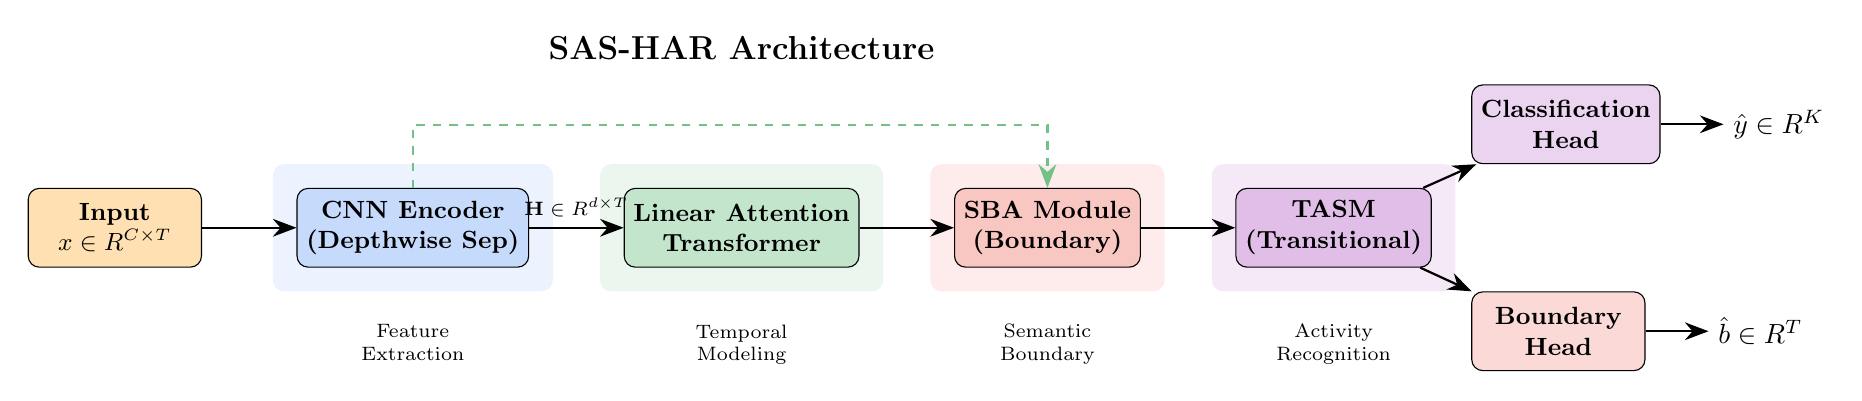
\begin{tikzpicture}[
    node distance=0.8cm and 1.2cm,
    block/.style={rectangle, draw, fill=#1, rounded corners, minimum height=1cm, minimum width=2.2cm, align=center, font=\small\bfseries},
    block/.default=white,
    arrow/.style={-{Stealth[length=3mm]}, thick},
    label/.style={font=\scriptsize, align=center}
]

% Input
\node[block=inputorange!30] (input) {Input\\$x \in \mathbb{R}^{C \times T}$};

% CNN Encoder
\node[block=cnnblue!30, right=of input] (cnn) {CNN Encoder\\(Depthwise Sep)};

% Transformer
\node[block=transformergreen!30, right=of cnn] (trans) {Linear Attention\\Transformer};

% SBA Module
\node[block=attentionred!30, right=of trans] (sba) {SBA Module\\(Boundary)};

% TASM
\node[block=headpurple!30, right=of sba] (tasm) {TASM\\(Transitional)};

% Output heads
\node[block=headpurple!20, above right=0.3cm and 0.5cm of tasm] (cls) {Classification\\Head};
\node[block=attentionred!20, below right=0.3cm and 0.5cm of tasm] (bnd) {Boundary\\Head};

% Final outputs
\node[right=0.8cm of cls] (cls_out) {$\hat{y} \in \mathbb{R}^{K}$};
\node[right=0.8cm of bnd] (bnd_out) {$\hat{b} \in \mathbb{R}^{T}$};

% Arrows
\draw[arrow] (input) -- (cnn);
\draw[arrow] (cnn) -- node[above, label] {$\mathbf{H} \in \mathbb{R}^{d \times T}$} (trans);
\draw[arrow] (trans) -- (sba);
\draw[arrow] (sba) -- (tasm);
\draw[arrow] (tasm) -- (cls);
\draw[arrow] (tasm) -- (bnd);
\draw[arrow] (cls) -- (cls_out);
\draw[arrow] (bnd) -- (bnd_out);

% Skip connection
\draw[arrow, dashed, transformergreen!70] (cnn.north) -- ++(0, 0.8) -| (sba.north);

% Background boxes
\begin{scope}[on background layer]
    \node[fit=(cnn), fill=cnnblue!10, rounded corners, inner sep=0.3cm] {};
    \node[fit=(trans), fill=transformergreen!10, rounded corners, inner sep=0.3cm] {};
    \node[fit=(sba), fill=attentionred!10, rounded corners, inner sep=0.3cm] {};
    \node[fit=(tasm), fill=headpurple!10, rounded corners, inner sep=0.3cm] {};
\end{scope}

% Labels
\node[above=1.5cm of trans, font=\large\bfseries] {SAS-HAR Architecture};

% Component descriptions
\node[below=0.6cm of cnn, label, text width=2.5cm] {Feature\\Extraction};
\node[below=0.6cm of trans, label, text width=2.5cm] {Temporal\\Modeling};
\node[below=0.6cm of sba, label, text width=2.5cm] {Semantic\\Boundary};
\node[below=0.6cm of tasm, label, text width=2.5cm] {Activity\\Recognition};

\end{tikzpicture}
\end{document}
